\documentclass[conference]{IEEEtran}
\IEEEoverridecommandlockouts
% The preceding line is only needed to identify funding in the first footnote. If that is unneeded, please comment it out.
\usepackage{cite}
\usepackage{amsmath,amssymb,amsfonts}
\usepackage{algorithmic}
\usepackage{graphicx}
\usepackage{textcomp}
\usepackage{xcolor}
\def\BibTeX{{\rm B\kern-.05em{\sc i\kern-.025em b}\kern-.08em
    T\kern-.1667em\lower.7ex\hbox{E}\kern-.125emX}}
\begin{document}

\title{Term Project Part 2 Report\\
{\footnotesize CENG 435 Data Communications and Networking}
}

\author{\IEEEauthorblockN{Dogancan Kartal}
\IEEEauthorblockA{\textit{Department of Computer Engineering} \\

\textit{Middle East Technical University}\\
Ankara, Turkey \\
e2036028@ceng.metu.edu.tr}
\and
\IEEEauthorblockN{Mert Bekar}
\IEEEauthorblockA{\textit{Department of Computer Engineering} \\
\textit{Middle East Technical University}\\
Ankara, Turkey \\
e2035749@ceng.metu.edu.tr}
}

\maketitle

\begin{abstract}
This document is aimed to give the reader an intuition about our progress for the second part of the term project of CENG435 course.
\end{abstract}

\begin{IEEEkeywords}
Reliable Data Transfer, ACK/NACK, Sequence Number, Pipelining, Multi-Homed Network, Checksum, Routing Table
\end{IEEEkeywords}

\section{Introduction}
In the second part of the term project, we again designed a network that consist of 5 nodes. A source node s, a broker b, two routers r1 and r2, and destination node d. We are tasked to send packets through the network and observe the experiments using several configurations. Packets are generated by source node and follows the path broker, one of the router and destination; Source to Broker via TCP and Broker to Destination via UDP based Reliable Data Transfer Protocol. Our main task is to implement the abovementioned UDP based Reliable Data Transfer Protocol.
\section{UDP based Reliable Data Transfer}
In the first part of the term project, even though we send our packets via UDP, which is an unreliable Transport Layer protocol, we didn't encounter any packet losses or bottlenecks on the network. The reason for that is: We waited for the ACK at the source node and send the next packet accordingly. There were no pipelining in this method. Since there were no pipelining, we had low utilization and much round trip times. This is one of the reasons why we are trying to implement a reliable data transfer protocol over UDP. We used the following mechanism to make the unreliable network reliable.
\subsection{Acknowledgement Mechanism}
Acknowledgement is a mechanism that specifies if the packet send from the sender node has been received from the receiver node correctly. The Acknowledgement Mechanism is first introduced at RDT 2.0. This is one of the main mechanisms that a reliable data transfer should have.
\subsection{Checksum Mechanism}
Checksum is a mechanism that allows us to understand if the packet send from the source node has been corrupted or not. Checksum is calculated with hash function according to the data content and the headers of the packet. After checksum is calculated on the source node, checksum is calculated again on the destination node and they are compared to understand if the packet is corrupted or not.
\subsection{Sequence Number Mechanism}
Sequence number is used for identifying the ordering of the packets in a pipelined system. Sequence number mechanism helps to identify the order of the bytes sent from one host to another so that the data can be reconstructed in order.
\subsection{Timeout Mechanism}
Timeout is a mechanism that allows the sender node to understand whether a packet is lost on the network or not. When the ACK is received at the sender node, we start a timer. If the timer exceeds the threshold we understand that the packet is lost in the network. When a threshold is set too low, there happens unnecessary retransmissions.  When a threshold is set too high, the source node waits too much to understand when a packet is lost. 
\subsection{Pipelining Mechanism}
Pipelining is mechanism that increases to overall utilization in the network by sending multiple packets from the sender node without waiting for their acknowledgements (i.e  stop-and-wait). There are 2 most-known techniques for that, Go-Back-N and Selective Repeat. We selected Go-Back-N for two reasons. First one is when a ACK is lost in the network, Go-Back-N handles this situation better than the selective repeat by not making lots of unnecessary retransmissions. Second reason is that the implementation of Go-Back-N at the destination node is simpler than the selective repeat since there is no extra buffer.
\subsection{Multi-Homing Mechanism}
Multi-homing is mechanism that splits the path of packets to more than one direction. It allows the broker node to split the load of the packets to the routers. It does this by not sending all the packets to the one of the routers but splitting their loads almost equally. It has some advantages. One of them is decreases the probability of bottleneck on the network. Multihoming mechanism also is prevents the problems when there happens a hardware problem on the one of routers. For example, if link is dead on the router 2, our RDT packet is sent again and it is guaranteed that the packet will be send to the destination from r1.
\section{Implementation}
\subsection{General Implementations}
\subsubsection{Source Node}
The main task of the source node is to read data from the file, divide the file into packets and send packets to the broker node over TCP. In the previous part of the term project, we waited for the ACK from the destination to send the next packet. But in this part, we send all the packets to the broker without waiting anything. Since it is stated in the homework text that a maximum size should be 1000 bytes, we choose 500 bytes per packet to make things simpler while calculating. We used previous configurations for the IP address (10.10.1.2) and port number (5000) for this part as well. We did not make too much implementation on the source node because its only interface is connected to the broker via TCP and it is already reliable.
\subsubsection{Broker Node}
The main task of the broker node is to receive packets from the source node and send them to the destination over routers with UDP based Reliable Data Transfer. Almost all of our implementations are done in the broker node. We used Queue data structure from the Queue module in the python. Queue module has 2 important methods that helps us very much which are $putnowait$ and $getnowait$. Our implementation is multithreaded, so we took advantage of these methods since there might happen a race condition between listening and sending events. These methods provide safe usage of the Queue.
\par We created 3 threads for the script that is running on the broker node. First thread listens the source node and puts the received data to the $msgs$ and $sndpkt$ queues. Second and third threads listen to the router 1 and router 2 nodes respectively. They wait for acknowledgements and when an ACK is received, the received ack is pushed to the $acks$ queue.
\par After creating threads, since we use Go-Back-N protocol, we send new packets after receiving ACKs. Because of this reason, the main process starts the timer and calls $rdtsend$ function to send the first $n$ packets where $n$ is equal to the window size. After that, main process calls $rdtrcv$ function. This function runs in an infinite loop. It applies Timeout Mechanism, Acknowledgement Mechanism and calls $rdtsend$ function. This function applies Sequence Number Mechanism and according to it, $rdtsend$ function gets the data to be send from the Queue, makes it packet and makes unreliable data send by using $udtsend$ function. $udtsend$ function applies Checksum Mechanism and Multi-Homing Mechanism and sends the packets.
\subsubsection{Destination Node}
The main task of the destination node is to receive packets from the routers, make the checksum and the return the acknowledgement. We use two threads, one for listening to router 1 and other for listening to router 2. We use some variables to implement Go-Back-N mechanism, to make these variables -will be discussed further- thread-safe, we use lock from the $threading$ module in python.
\subsection{Acknowledgement Mechanism}
We mentioned the advantages of ACK mechanism for our purposes above. We handled ACK mechanism by checking the received packet from the routers at Broker Node. When we receive an ACK, we understand that the current packet has been delivered by the Destination Node without corruption.
\subsubsection{Source Node}
Since Source Node is connected to broker via TCP, there is no need to implement ACK mechanism there.
\subsubsection{Broker Node}
In Broker Node, we put the received ACKs to the $acks$ queue in order to make it thread-safe since we listen from both router 1 and router 2. 
\subsubsection{Destination Node}
In Destination Node, we understand if a packet corrupted in the network by using checksum mechanism and if it is not corrupted we return an ACK to tell the Broker Node that we received correctly.
\subsection{Checksum Mechanism}
We mentioned the advantages of checksum mechanism for our purposes above. We handled checksum mechanism by using hash functions provided by $MD5$ module of python.
\subsubsection{Broker Node}
We calculated 16 byte hash value of payload and the headers by using $MD5$ module methods which are $MD5.update()$ and $MD5.digest()$. After this calculation, we put the checksum to the payload of packet to be processed by the destination despite UDP header have field for checksum. To put checksum value into UDP header,  we had to use $rawsocket$, so we put checksum value into payload of packets. 
\subsubsection{Destination Node}
At destination node, we first extract the original checksum value of the received packets' payload. Then, we calculate the checksum using payload and the header of the received packet. We then compare these checksums. If they are same, we understand that the packet is not corrupted in the network.
\subsection{Sequence Number Mechanism}
The details of the implementation of the sequence number mechanism is described in depth in the pipelining mechanism subsection.
\subsection{Timeout Mechanism}
We mentioned the advantages of timeout mechanism for our purposes above. We handled timeout mechanism by starting and stopping timers and using the threshold value that we sad.
\subsubsection{Broker Node}
In Broker Node, we started the time when the first packet of the window is sent and when we receive an acknowledgement. We choose threshold value $0.2$ second. When we make the threshold value lower or higher, we observed that the total file transmission time increases. So, $0.2$ second is optimum for us. Also, timeout mechanism is uses by pipelining mechanism which we will discuss later. If the timer exceeds our threshold value, we understand that the packet is lost in the network.
\subsubsection{Destination Node}
The implementation of timeout mechanism applies only for broker node.
\subsection{Pipelining Mechanism}
We choose Go-Back-N as a pipelining mechanism. We mentioned the advantages of pipelining mechanism and Go-Back-N for our purposes above. To implement Go-Back-N (GBN) mechanism, we followed a similar path for given in Figure 1 for the Broker Node and Figure 2 for the Destination Node. 
\begin{figure}[t]
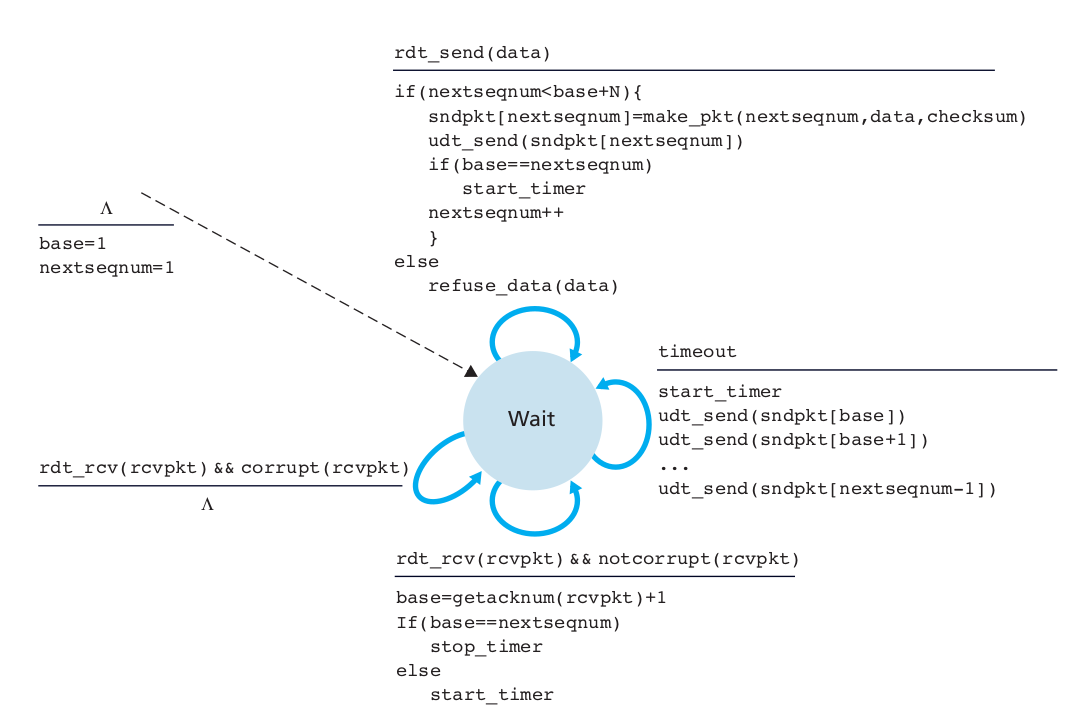
\includegraphics[width=8.5cm, height=7cm]{gbn_sender.png}
 \caption{GBN Sender State Machine}
 \label{fig:1}
\end{figure}
\begin{figure}[t]
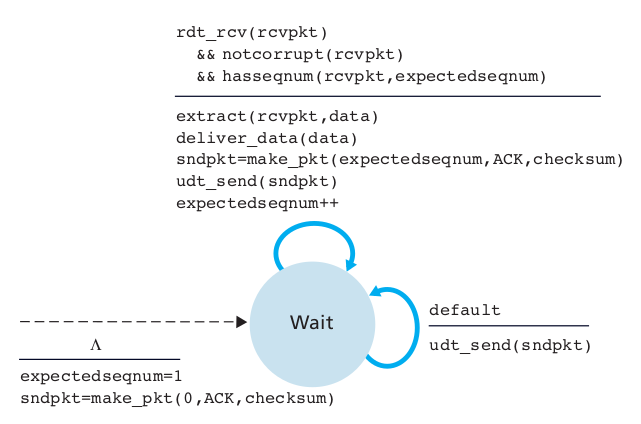
\includegraphics[width=8.5cm, height=7cm]{gbn_receiver.png}
 \caption{GBN Receiver State Machine}
 \label{fig:1}
\end{figure}
\subsubsection{Broker Node}
GBN uses windows to send packets. The purpose for this is to increase the utilization. For any given time, there are maximum number of packets equal to the window size. We set our window size to 5. Setting smaller window size makes the utilization smaller because there a less number of packets on the given for any given time. Setting bigger window size makes the number of retransmission more because when a packet is lost, whole packets from the lost packet to the end of window is sent again.
\par We have $base$ and $nextseqnum$ variables. $base$ is the sequence number of the first packet of the current window. $nextseqnum$ is the sequence number of the next packet to be sent later. Broker node controls the timeout mechanism and checks the received ACK. If the received ACK is bigger than the $base$, which is the first sent packet of the current window, it means that some of the ACKs in the network are lost and selecting Go-Back-N protocol helps us to not retransmit the intermediate packets. In this case, base is updated $ACK+1$ and $rdtsend$ function is called. In case of equality to the $base$, everything is as expected and $rdtsend$ function is called.  $rdtsend$ function, when called, checks whether there are any unsent packet in the window by: \texttt{nextseqnum < base + n} and if there is, it gets the data to be send from the Queue, makes it packet and makes unreliable data send by using $udtsend$ function.
\subsubsection{Destination Node}
In the destination node, to implement GBN, we keep a variable called $expectedseqnum$. This variable keeps cumulative sequence number about the received packets. When the destination node receives a packet, it extracts the sequence number from the packet and checks whether it is equal to the  $expectedseqnum$ or not. If they are same, we can understand that the packet is received with the correct order and we send immediately the ACK of the current packet. If they are not same, we can understand that the packet is received with the incorrect order and send immediately the ACK of the lastly true-order received packet to give the broker node cumulative information about the orderly received packets. 
\subsection{Multi-Homing Mechanism}
We mentioned the advantages of multi-homing mechanism for our purposes above. We randomly choose one of the two routers, one is selected randomly. At the end of the experiment, number of packets sent to each router converges to 50 percent. 
\subsubsection{Broker Node}
On the Broker Node, we have to choose path for each packet. There are two possible pathes, first one is $Broker-R1-Destination$ and second is $Broker-R2-Destination$. We selected one of them randomly. For this, we use $random$ module of python. We sent packets to routers according to result of randomly select. 
\subsubsection{Destination Node}
Destination Node listens each of routers, r1 and r2 because of multi-homing mechanism. It gets packets from these routers and puts payloads of packets into $receivedfile$ list.
\section{Configuration of Routing Tables}
In the first part of this project, we run scripts for each router to delivers packets. However, running scripts on the router conflicts the purpose of usage of the routers. Routers have a routing table which provide packet transfer from one node to another node as fast as possible. Therefore, we used routing table on R1 and R2 Node instead of running script.
\par Each router must have a capability of providing a two way packet forwarding. Therefore, we have to put 2 entry on routing table for each router. First one should forward the packets from Broker Node to Destination Node and second one should forward the packets from Destination Node to Broker Node. We use \texttt{route} commands to put entry on routing table. This is the general form of the \texttt{route} commands: \\
\texttt{sudo route add -net "Dest IP" netmask "Netmask Config" gw "Forwarding IP"} \\
We have to manipulate 3 field in this general form of \texttt{route} command. 
\begin{itemize}
    \item Dest IP: This field represents the destination IP address of incoming packets to router.
    \item Netmask Config: Incoming packet match the entry according to this entry. It can be between $0.0.0.0$ and $255.255.255.255$. If it equals to $255.255.255.255$, destination IP of packets must be same with "Dest IP" field to match with that entry.
    \item Forwarding IP: This field represents which IP address the packets will be forwarded.
\end{itemize}
We use following commands for put an entry to routing table for each router. 
\begin{itemize}
    \item R1 Node: 
        \begin{itemize}
            \item Forwarding packets to Destination Node from Broker Node. \\
            \texttt{sudo route add -net 10.10.3.2 netmask 255.255.255.255 gw 10.10.3.2}
            \item Forwarding packets to Broker Node from Destination Node. \\
            \texttt{sudo route add -net 10.10.2.1 netmask 255.255.255.255 gw 10.10.2.1}
        \end{itemize}
    \item R2 Node: 
        \begin{itemize}
            \item Forwarding packets to Destination Node from Broker Node. \\
            \texttt{sudo route add -net 10.10.5.2 netmask 255.255.255.255 gw 10.10.5.2}
            \item Forwarding packets to Broker Node from Destination Node. \\
            \texttt{sudo route add -net 10.10.4.1 netmask 255.255.255.255 gw 10.10.4.1}
        \end{itemize}
\end{itemize}

\section{Experiment Observations}
As mentioned above, the main task of this part of the term project is to make a unreliable network reliable. Packet loss, corruption and reordering are 3 of the most core concepts that a reliable network should handle. We made all of the experiments and plotted their graphs accordingly. In order to observe the behaviour of our protocol, we made each of the experiment $20$ times.
\subsection{Packet Loss}
The main task of this experiment is to observe whether our UDP based reliable data transfer protocol is able to handle the packet loss situation with different configurations or not. We run the following commands for the nodes between Broker and Destination Nodes with changing $loss$ value according to desired values, $0.5\%$, $10\%$ and $20\%$:
\begin{itemize}
    \item Broker Node: \\
        \texttt{sudo tc qdisc add dev eth1 root netem loss 0.5\% corrupt 0\% duplicate 0\% delay 3 ms reorder 0\% 0\%} \\
        \texttt{sudo tc qdisc add dev eth3 root netem loss 0.5\% corrupt 0\% duplicate 0\% delay 3 ms reorder 0\% 0\%}
        \item R1 Node: \\
        \texttt{sudo tc qdisc add dev eth1 root netem loss 0.5\% corrupt 0\% duplicate 0\% delay 3 ms reorder 0\% 0\%}
        \item R2 Node: \\
        \texttt{sudo tc qdisc add dev eth2 root netem loss 0.5\% corrupt 0\% duplicate 0\% delay 3 ms reorder 0\% 0\%}
\end{itemize}
\par We set to \texttt{INTERFACE} field according to data flow. We choose left side interface of all links between Broker Node and Destination Node as a \texttt{INTERFACE}. We set the packet loss percentage $0.5\%, 10\%, 20\%$ respectively.
\par Setting the packet loss parameters means that specified link drops the packet that it carries with the given percentage. We used timeout mechanism to handle the packet loss. More details are mentioned in the above  \texttt{Timeout Mechanism} subsections in the \texttt{UDP Based Reliable Data Transfer} and \texttt{Implementation} sections.
\par We expect that the file transfer time increases when the packet loss percentage increases. The reason for that is, we wait for $0.2$ seconds to understand if a packet is lost and make retransmissions when necessary. Also, we expect that each data of the file is received and reconstructed at the destination node.
\par Given in Figure 3, we observed our expectations. We observed that the file transfer time increased as the probability of packet loss increases. Retransmission is the main reason for this. Moreover, we reconstructed the packets data to the exact input file. To understand this, we used $diffchecker.com$ and validated that two files are identical.

\begin{figure}[t]
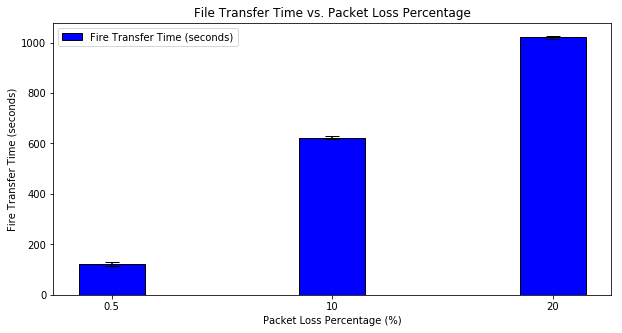
\includegraphics[width=8.5cm, height=7cm]{experiment-loss.png}
 \caption{Packet Loss Experiment}
 \label{fig:1}
\end{figure}
\subsection{Corruption}
The main task of this experiment is to observe whether our UDP based reliable data transfer protocol is able to handle the packet corruption situation with different configurations or not. We run the following commands for the nodes between Broker and Destination Nodes with changing $corruption$ value according to desired values, $0.2\%$, $10\%$ and $20\%$:
\begin{itemize}
    \item Broker Node: \\
        \texttt{sudo tc qdisc add dev eth1 root netem loss 0\% corrupt 0.2\% duplicate 0\% delay 3 ms reorder 0\% 0\%} \\
        \texttt{sudo tc qdisc add dev eth3 root netem loss 0\% corrupt 0.2\% duplicate 0\% delay 3 ms reorder 0\% 0\%}
        \item R1 Node: \\
        \texttt{sudo tc qdisc add dev eth1 root netem loss 0\% corrupt 0.2\% duplicate 0\% delay 3 ms reorder 0\% 0\%}
        \item R2 Node: \\
        \texttt{sudo tc qdisc add dev eth2 root netem loss 0\% corrupt 0.2\% duplicate 0\% delay 3 ms reorder 0\% 0\%}
\end{itemize}
\par We set to \texttt{INTERFACE} field as mentioned packet loss experiment. We set the corruption percentage $0.2\%, 10\%, 20\%$ respectively.
\par Setting the corruption parameters means that specified link corrupts the packet that it carries with the given percentage. We used checksum mechanism to handle the packet corruption. More details are mentioned in the above  \texttt{Checksum Mechanism} subsections in the \texttt{UDP Based Reliable Data Transfer} and \texttt{Implementation} sections.
\par We expect that the file transfer time increases when the corruption percentage increases. The reason for that is, when we receive corrupted packet in the Destination Node, the Destination Node sends 
previously correctly received packets' ACK. When the Broker Node receives a duplicate ACKs, it waits for timeout for a given threshold and it triggers making retransmissions. Also, we expect that each data of the file is received and reconstructed at the Destination Node.
\par Given in Figure 4, we observed our expectations. We observed that the file transfer time increased as the probability of corruption increases. Retransmission is the main reason for this. Broker Node waits for timeout when it receives duplicate ACKs because we did not implement fast retransmission mechanism. Moreover, we reconstructed the packets data to the exact input file. To understand this, we used $diffchecker.com$ and validated that two files are identical.
\begin{figure}[t]
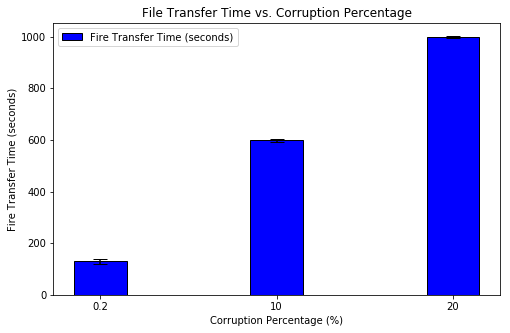
\includegraphics[width=8.5cm, height=7cm]{experiment-corrupt.png}
 \caption{Corruption Experiment}
 \label{fig:1}
\end{figure}
\subsection{Reorder}
The main task of this experiment is to observe whether our UDP based reliable data transfer protocol is able to handle the packet reordering situation with different configurations or not. We run the following commands for the nodes between Broker and Destination Nodes with changing $reorder$ value according to desired values, $1\%$, $10\%$ and $35\%$:
\begin{itemize}
    \item Broker Node: \\
        \texttt{sudo tc qdisc add dev eth1 root netem loss 0\% corrupt 0\% duplicate 0\% delay 3 ms reorder 1\% 50\%} \\
        \texttt{sudo tc qdisc add dev eth3 root netem loss 0\% corrupt 0\% duplicate 0\% delay 3 ms reorder 1\% 50\%}
        \item R1 Node: \\
        \texttt{sudo tc qdisc add dev eth1 root netem loss 0\% corrupt 0\% duplicate 0\% delay 3 ms reorder 1\% 50\%}
        \item R2 Node: \\
        \texttt{sudo tc qdisc add dev eth2 root netem loss 0\% corrupt 0\% duplicate 0\% delay 3 ms reorder 1\% 50\%}
\end{itemize}
\par We set to \texttt{INTERFACE} field as mentioned packet loss experiment. We set the reorder percentage $1\%, 10\%, 35\%$ respectively.
\par Setting the reorder parameters means that specified link corrupts the packet that it carries with the given percentage. We used sequence number mechanism to handle the packet reordering. More details are mentioned in the above  \texttt{Sequence Number Mechanism} and \texttt{Pipelining Mechanism} subsections in the \texttt{UDP Based Reliable Data Transfer} and \texttt{Implementation} sections.
\par We expect that the file transfer time increases when the reordering percentage increases like above experiments. When we received an unordered packets at the Destination Node, Destination Node send a previously ordered received packets' ACK. When the Broker Node receives duplicate ACKs, we expect long delays at the network because our protocol does not support fast retransmission. Also, we expect that each data of the file is received and reconstructed at the destination node.
\par In Figure 5, we plotted the File Transfer Time vs. Reordering Percentage graph. It can be observed that the differences are not like the previous experiments, they are smaller. Before this experiment, we expected that the file transfer time increases when the reordering percentage increases but we did not observe it. Since we picked our window size = 5 and link delay = 3, there is not a lot of packet flowing on the network at the same time. Reorder parameter in the netem tc command reorders packet on the current link. We didn't observe a lot of difference when we increase the reorder percentage because there is not a lot of packets on a link to be reordered. To see if we were correct about our assumptions, we set the link delay to 30ms and observed that there happens lots of more reordered packets since there are more packets on the network at the same time. Moreover, we reconstructed the packets data to the exact input file. To understand this, we used $diffchecker.com$ and validated that two files are identical.
\begin{figure}[t]
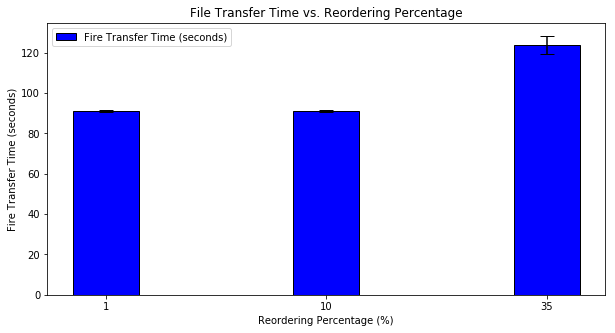
\includegraphics[width=8.5cm, height=7cm]{experiment-reorder.png}
 \caption{Reordering Experiment}
 \label{fig:1}
\end{figure}
\section{Conclusion}
To conclude, we constructed a network that handles the duties of main features of the UDP based reliable data transfer protocol which are Acknowledgement Mechanism, Checksum Mechanism, Sequence Number Mechanism, Timeout Mechanism, Pipelining Mechanism and Multi-Homing Mechanism. In the first part of the term project, we constructed a network with TCP and UDP. Because of the bottleneck, we observed lots of packet losses since UDP is not reliable and we didn't have a mechanism to handle this other than waiting for an ACK. Our UDP based reliable data transfer protocol handled reliability problems of UDP faster than our solution in first part of term project. In this part, we took advantage of multithreading and Queue data structure for our implementation. We configured the routing table of routers, R1 and R2. Our UDP based reliable data transfer protocol can handles packet loss, corruption and reordering situations. It could also transfer file correctly. We ensured reliability of our protocol with doing three experiments; Packet Loss Experiment, Corruption Experiment and Reordering Experiment. We made each experiments 20 times and observed our protocol's reaction to the packet loss, corruption and reordering. We also plotted a graph for each experiments and these graphs support reliability of our protocol. Each result of the experiments are given in the $experiments.py$ file.
\end{document}
